\section{Data Models and Metadata}

\subsection{Models Catalogue}

A software \emph{model} is an abstraction of a software program, which
will be instantiated and run using \emph{real data}, software
modelling is becoming important for a number of reasons, not least
that it enables developers the opportunity to \emph{re-use} code. The
Unified Modelling Language UML \cite{UML} or Ecore \cite{ECORE} ( a
subset of UML) are in widespread use for defining and representing
software \emph{models}. UML and Ecore are defined at a level which is
\emph{more abstract} than the model itself, and one which we term the
\emph{meta-modelling} layer.

Thus there are two things we need to identify and reference in
building the toolkit, firstly does this \emph{concept} \textbf{mean}
the same as that \emph{concept}, and secondly does this \emph{concept}
have the same \emph{representation} as that concept. The way in which
we can match up concepts in software engineering is by associated them
with classes of software objects, and then defining methods which can
reference them.

\subsection{Model Driven Software Engineering (MDSE)}

Clinical research data is stored in many different formats, and data
which may needed for a study may well originate in many different
places. As well as the precise semantics of the data being difficult
to capture, so to is the syntax. One set of forms may have been
captured using Excel, another using a web-based service such as Survey
Monkey, and yet another is stored in a relational database. The
majority of data comes either from a patient answering a question and
recording the answer on some kind of electronic form representation or
from a clinician answering a question and recording the answer. Many
questions will be similar, for instance \emph{what is the patient's
  weight at a particular time}, but they may have different conditions
attached \emph{after a meal, before taking the medicine}. The problem
when dealing with datasets with such research results is that the
structure of the data varies. Collecting data together for the
purposes of running federated queries across the data is largely a
structural rather than a behavioural problem. MDSE is a branch of
computer science which treats the \emph{model} as the primary object
of study. It also is able to transform data from it's stored
structure, with transformation languages such as ATL ~\cite{ATL}, XSLT
~\cite{XSLT} and QVT ~\cite{QVT} data can be transformed from one
format to another format for use in different systems. MDSE provides
the theoretical background which enables these transformations to be
designed and used in code generation toolkits and in
semi-automatically generated software toolkits.

\subsubsection{Metadata and ISO11179}
ISO11179 is the international standard relating to metadata and in particular metadata registries. The ideas and principles documented in this standard have informed the development of the models catalogue from the early prototypes built as part of the Cancer Grid project \cite{crichton2009metadata}, through to the latest versions of the models catalogue.

\begin{figure}[here]
	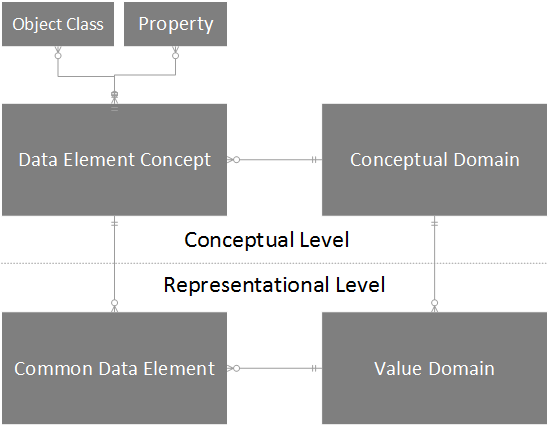
\includegraphics[width=0.48\textwidth,natwidth=610,natheight=642]{BasicISO}
	\caption{Core model for ISO11179 Metadata Registry} 
	\label{fig:basicMDR}
\end{figure}

The ISO11179 standard uses the notion of a \emph{data element concept}, \emph{a data element}, \emph{a value domain}, and a \emph{conceptual domain}. The standard currently confines itself to the detailed level of concepts and data elements and has no notion of collections of data elements or data element concepts, but instead attaches two attributes: an \emph{object class} and a \emph{property} to each data element concept and these attributes allow the data element concept's to be aggregated or classified. This core model of the ISO11179 is illustrated in figure \ref{fig:basicMDR}. The data element concept and conceptual domain entities belong to the \emph{conceptual level}  whilst the common data element and value domain both belong to the \emph{representational level}.


For example an Integer data-type in a programming language may be used to represent inches in a measurement program, it may also be used to count vehicles in a logistics application.  A data element is said to be comprised of a data element concept(DEC) which is its meaning and a value domain(VD) which is its representation.

\begin{table}[h]
	\begin{tabular}{ p{1.8cm} p{2.8cm}  p{3.0cm}  }  % centered columns (2 columns)
		\hline
		Entity & ISO Definition & ISO11179 Implementation Guidelines  \\ 
		\hline
		Data Element Concept(DEC) & An idea that can be represented in the form of a data element, described independently of any particular representation. & A concept that can be represented in the form of a Data Element, described independently of any particular representation.\\
		Common Data Element(CDE) & A unit of data for which the definition, identification, representation, and permissible values are specified by means of a set of attributes. & A unit of data for which the definition, identification, representation and Permissible Values are specified by means of a set of attributes. \\
		Value Domain (VD) & The description of a value meaning. & A description of a Value Meaning. \\
		Conceptual Domain (CD) & A set of valid value meanings, which may be enumerated or expressed via a description.& A set of valid Value Meanings.\\
		\hline
	\end{tabular}
\end{table}

The table lists the definitions of the key entities used in the standard
Conceptual domains comprise sets of value domains, they provide a collection mechanism of \emph{Value Meanings} which provide representation for a particular data element concepts. Data Element Concepts can then be grouped according to their Object Class, or Property, however whilst this works for a system that is focussed entirely on the metadata units, any working software system will need to group the data elements in a structure that is easily transformed into the components such as Classes and Entities that are used in most information systems.   



\subsection{Data Modelling and Meta-Modelling}
In our work with clinical trials the metadata registry standard on its own is insufficient to answer our principle use cases, which were to share data models, encourage re-use of data elements where possible, develop new data models, and use those data-models in the generation of software artefacts in particular forms for clinical trials.

Working with the ideas captured in the standard and applying them to our use cases we have developed a \emph{domain specific language for meta-modelling} which internally we are calling LEMMA; it is essentially a domain specific language which was developed for handling of clinical research data, but which could possibly be used in other domains. As a computer language it is  weak, however the main problem we are using it for is to restructure clinical \emph{data-models} and for the task in hand it has proved capable.

The key concept behind the language is that of a datamodel, a datamodel is a model composed of dataclasses and dataelements which holds structured data in a particular subject area. The \emph{models catalogue} toolkit is essentially a registry for these \emph{datamodels}, each one being registered with a version number. The datamodel maintains the structure and relationships between a set of dataclasses and dataelements, each of which essentially represent a \emph{data concept}. Dataclasses are in essence very similar to \emph{entities} in entity-relational diagrams, and to \emph{classes} in object-orientated programming; they are simply data-structures. They can be composed from other dataclasses, or from dataelements. Dataelements are atomic entities which can represent a concept or a component of a concept, they can exist in a datamodel independently or as a compositional attribute inside a dataclass. We have a built a version of the language using the Eclipse Modelling Framework (EMF ~\cite{EMF}), basing the various entities on Ecore~\cite{ECORE} classes. A simplified overview model, without attributes and methods, showing the Ecore model for this DSL is shown in Figure \ref{fig:mcSimplifiedOverview}.
%%------------REDO-----------------------%%
\begin{figure}[here]
	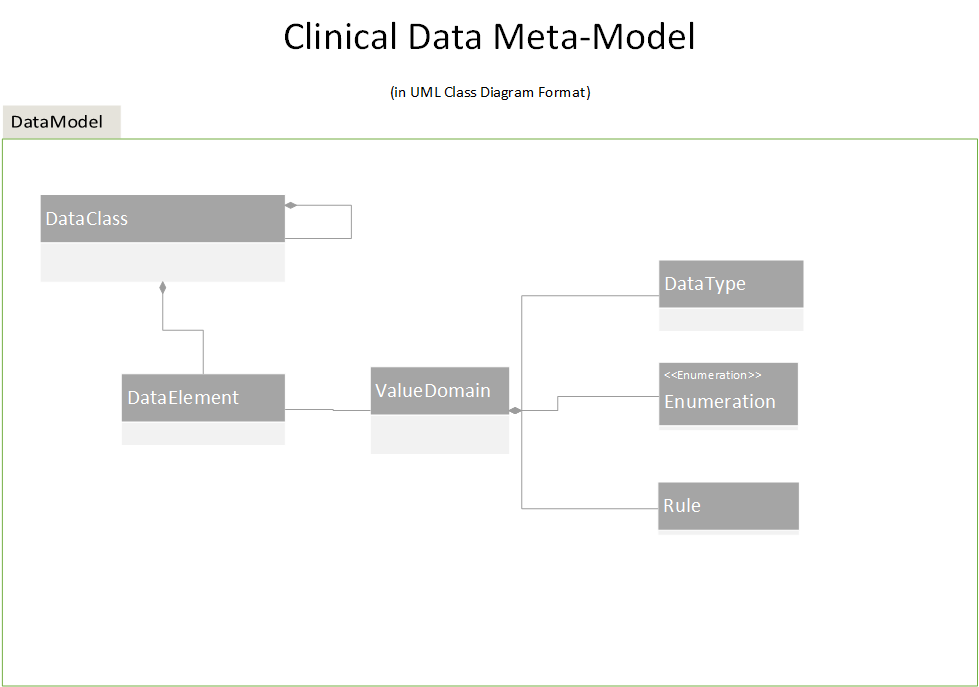
\includegraphics[width=0.5\textwidth,natwidth=610,natheight=642]{MetaModel}
	\caption{Overview of Metamodel} 
	\label{fig:mcSimplifiedOverview}
\end{figure}

\subsubsection{DataModel}
A datamodel is a grouping or containment entity which groups a set of \emph{DataClasses} together. DataModels can be thought of as datasets, or even database schemas, very often in the medical domain they are defined either by XML Schema definition files, or by equivalent schemas written in Excel. 
DataModels are collections of \emph{ConceptElements} which in turn can be either \emph{Data Elements} or \emph{Classes}. There is no real notion of composition or multiplicity, a instance of a DataModel can contain an instance of a Data Element or not as required by the instance.  DataModels are named, have a description and have a version identity.
\subsubsection{DataClass}
A DataClass is a grouping or collection of \emph{attributes} which can be data elements or classes, the attributes are currently \emph{mandatory}, so that DataClass with 5 attributes must have those 5 attributes instantiated in an instance for it to be considered of that DataClass. A DataClass in our meta-modelling language is so named to differentiate it from the term \emph{Class} as used in object oriented programming languages, the main difference being that it captures the structural rather than behavioural aspects of a class.  DataClasses represent \emph{Concepts}, and can be \emph{Generalized} into a hierarchy, giving some of the benefits of inheritance to the language. In essence it enables users to take dataclasses from one datamodel, build a sub-class with all the previous data points and then add to it with new dataclasses and dataelement.
\subsubsection{Data Elements} 
Data Elements can also represent \emph{Concepts} and are by their nature \emph{atomic}.  Each data element is related to a value domain on a one-to-one basis, and the relationship is a two-way relationship.
\subsubsection{Value Domain}
A Value Domain is the domain in which the data element is represented, it can consist of one or more \emph{ValueSpecs}. In addition a valuedomain can have zero or more \emph{Measurement Units}, which are descriptive tags which refer to a measurement unit such as kilometers per hour, imperial pounds, or meters. 
\subsubsection{ValueSpec}
ValueSpecs are intermediate entities to describe \emph{how} the data will be represented. There are 3 ValueSpecs, the first is a \emph{datatype}, the second is an \emph{enumeration} of a datatype, and the last is a \emph{rule}. A valuedomain will have at least one ValueSpec and at most 3 ValueSpecs which must be of different kinds.
The main reason for creating a language for handling the data structures in this manner is not only so that models can be curated, versioned and maintained easily, but that the datamodels produced can then be transformed automatically for use in other heterogeneous systems. To illustrate this figure ~\ref{fig:mofLayers} shows the LEMMA meta-model within a 4 tier abstraction diagram. The layers within this diagram are based around idea put forward by the  OMG(~\cite{OMG}), specifically model driven architecture (MDA ~\cite{MDA}). The MDA defines \emph{n} abstraction layers for modelling, although 4-layers are normally used.
\begin{figure}[here] 
	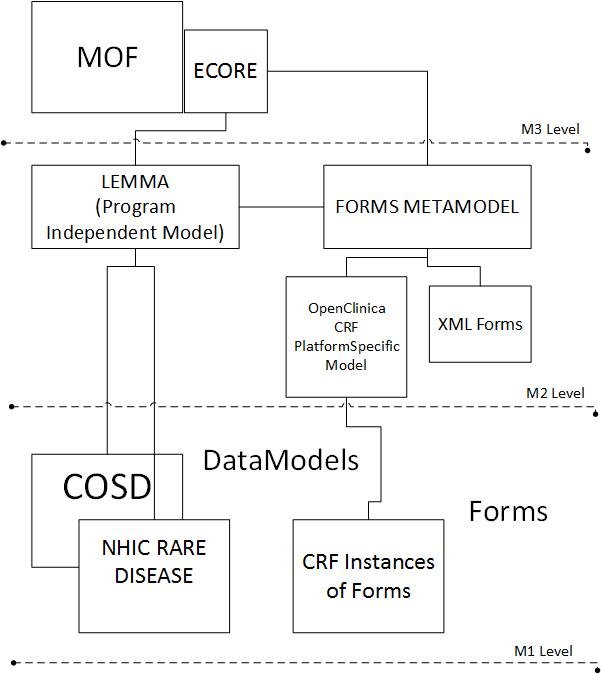
\includegraphics[width=0.5\textwidth,natwidth=610,natheight=642]{MOFLayers}
	\caption{ Datamodel in Excel Format} 
	\label{fig:mofLayers}
\end{figure}
The M0 layer is \emph{real-world} level, the level at which real world objects exist, people, cars, programs, etc. The M1 layer is level at which programs, such as a java program, or a java class definition exist in their static runtime form. The instantiation of a class occurs at the level below the class, so a java object runs in level M0. In defining datasets or datamodels we are dealing in datamodels which are instantiated at the M1 level, the \emph{Cancer and Outcomes Services Dataset} exists at this level, although their may be many conforming instances running at the M0 level. The datamodel is defined in out meta-modelling language, which exists at the M2 or meta-modelling level, and in turn conforms to the more abstract specification known as ECore.

An instance of a datamodel can be written in this DSL in the same way as java code, and figure \ref{fig:excelCOSD} shows how this code looks in the eclipse development toolkit. In this diagram the excel representation of the \emph{Cancer and Outcomes Services Dataset} shown in figure \ref{fig:excelCOSD} has been transformed into the meta-model.

\begin{figure}[here]
	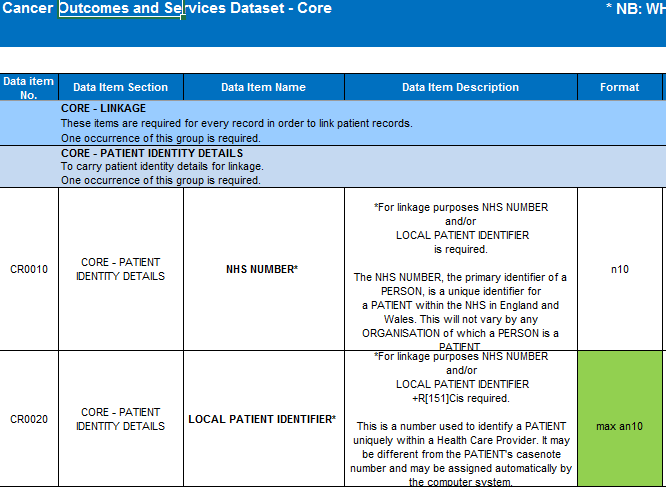
\includegraphics[width=0.5\textwidth,natwidth=610,natheight=642]{COSDExcelS}
	\caption{ Datamodel in Excel Format} 
	\label{fig:excelCOSD}
\end{figure}
The DSL is used to represent a model for Cancer data (part of the Cancer Outcomes and Services Dataset ~\cite{COSD}) in figure \ref{fig:elmcosd}, and is being used within the eclipse toolkit. The DSL can be used to transfer datasets between instances of the models catalogue, although other formats such as JSON and XML are also available.

\begin{figure}[here]
	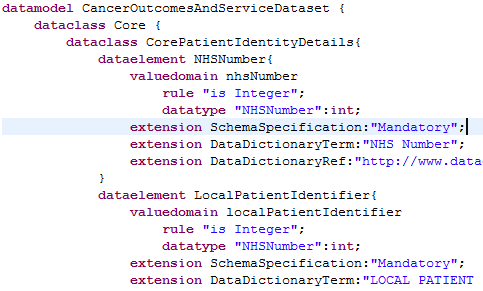
\includegraphics[width=0.5\textwidth,natwidth=610,natheight=642]{MCCOSDModelS}
	\caption{ Datamodel in Eclipse environment} 
	\label{fig:elmcosd}
\end{figure}

\subsection{Forms and Automatic Software Generation}

By defining the LEMMA metamodel and a similar and dependent Forms metamodel, both at the M" level, and both \emph{Platform Independent} we are able to relate curated data elements to forms elements, and by selecting a group of dataelements and dataclasses automatically generate a set of related forms. This can be done in several ways, the most used way is to generate a platform independent model and then use that model to generate an Excel template. 


